% GENERATED by tools/render_sysml_diagrams.py. Do not edit: the next run overwrites it.
% To change a caption, edit the `// caption:` line above the view in the .sysml file.
% To add or remove a figure, add or remove the view in the model.
% To move a figure between the body and the appendix, add or remove a
% `// placement: body` line above the caption line.

\begin{landscape}
\begin{figure}[!htbp]
\centering
\pdfimageresolution=300
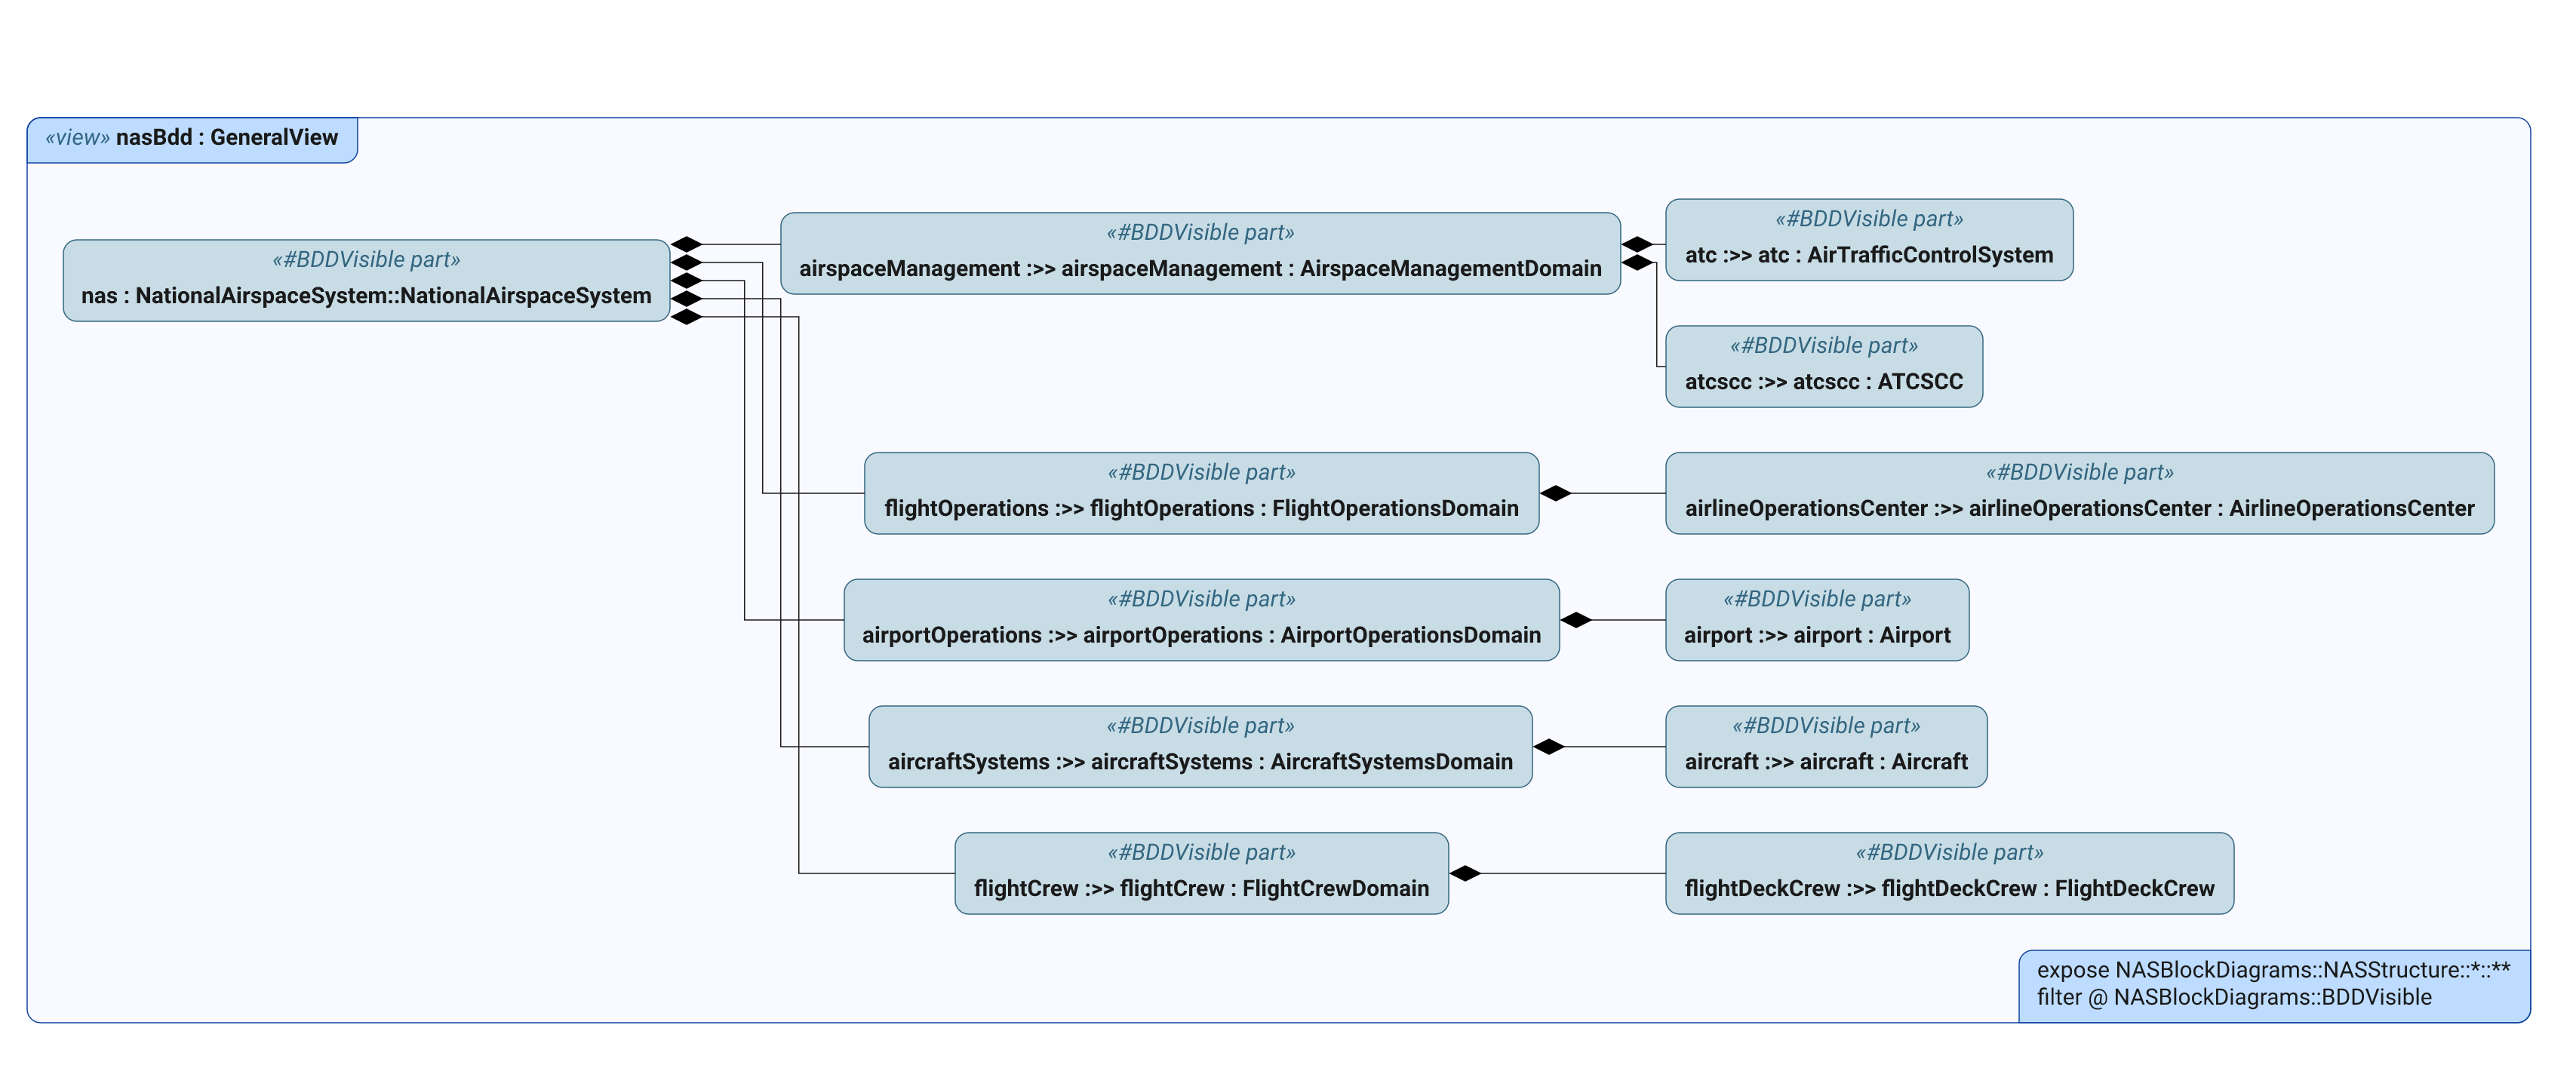
\includegraphics[width=\linewidth,height=0.8\textheight,keepaspectratio]{sysml/diagram-nasBdd}
\caption{NAS block definition diagram: the modeled domains and the context-diagram systems, composition only. View \texttt{nasBdd}; source \texttt{nas\_block\_diagrams.sysml}; rendered 2026-10-19.}
\label{fig:sysml-nasBdd}
\end{figure}
\end{landscape}

\begin{landscape}
\begin{figure}[!htbp]
\centering
\pdfimageresolution=300
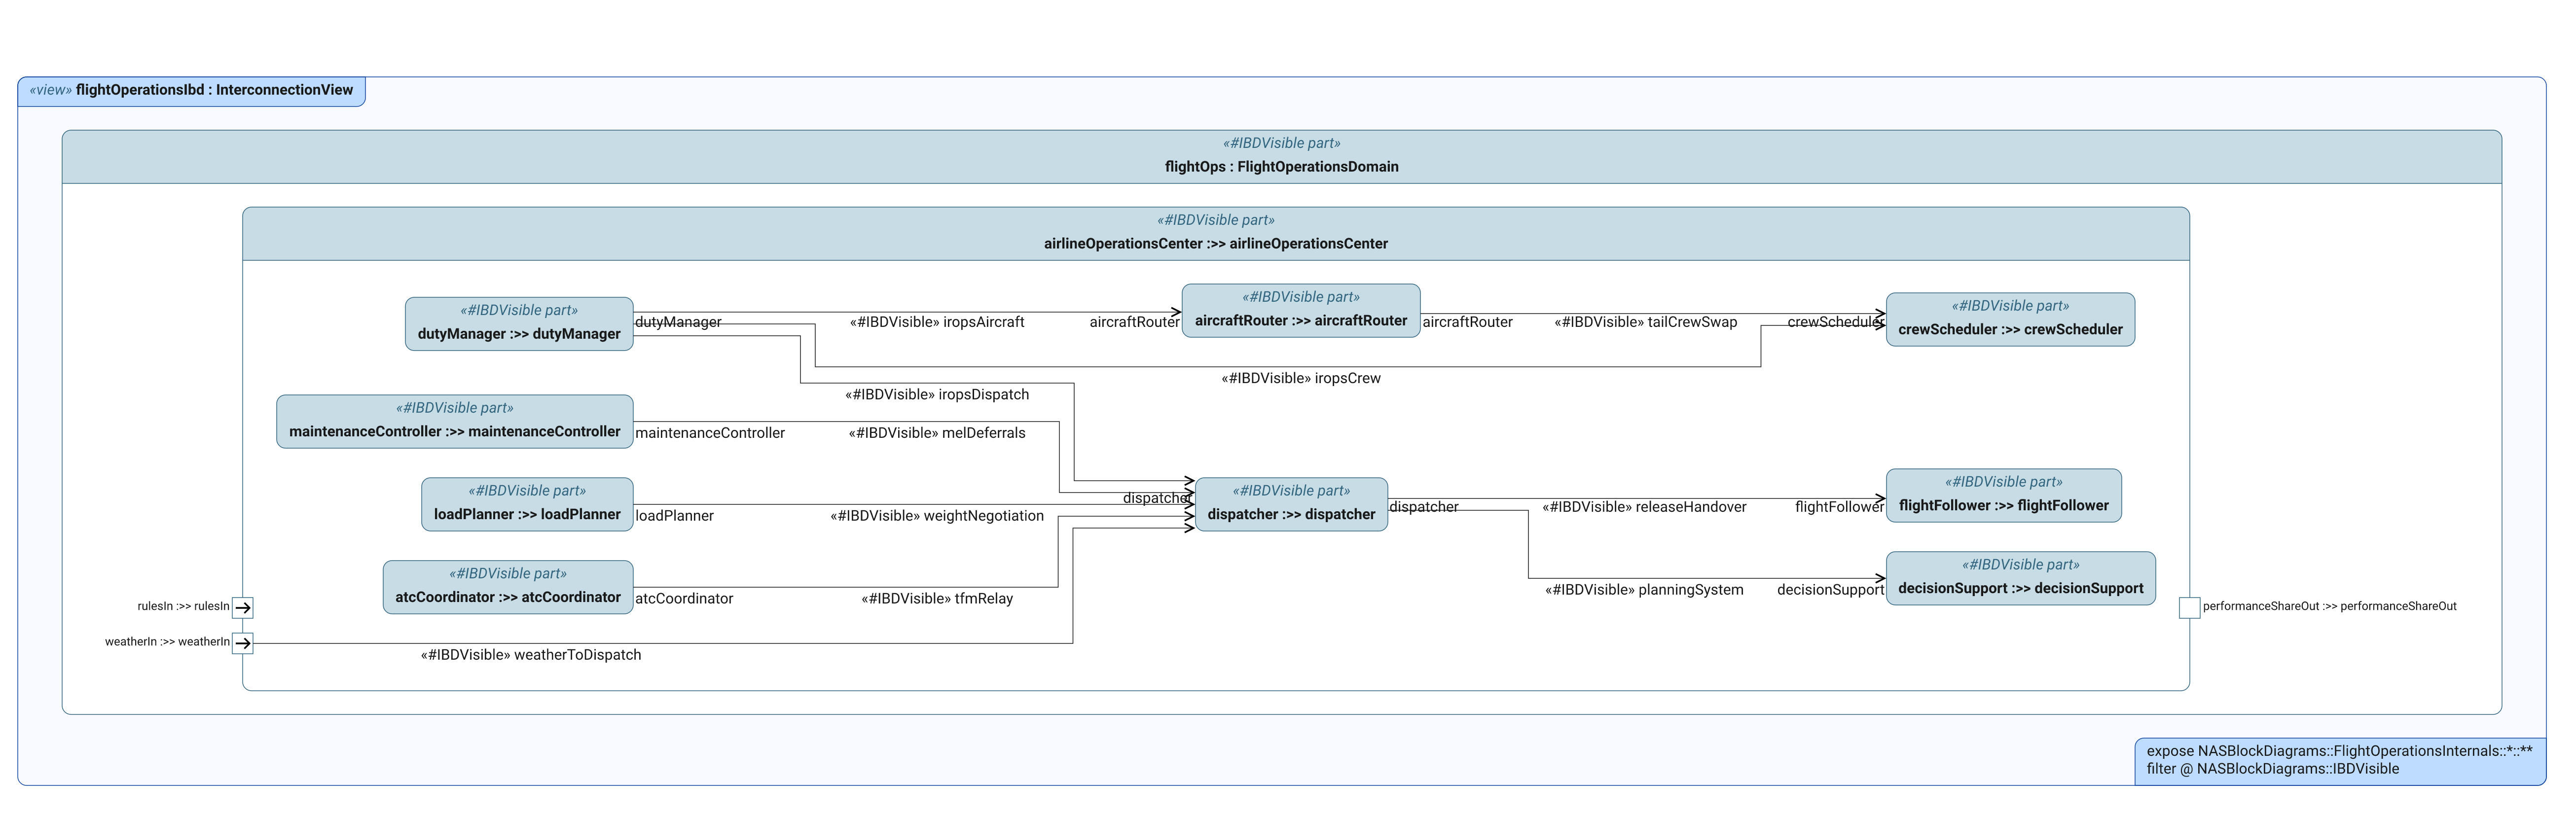
\includegraphics[width=\linewidth,height=0.8\textheight,keepaspectratio]{sysml/diagram-flightOperationsIbd}
\caption{Flight operations internal block diagram: the airline operations center's roles. View \texttt{flightOperationsIbd}; source \texttt{nas\_block\_diagrams.sysml}; rendered 2026-10-19.}
\label{fig:sysml-flightOperationsIbd}
\end{figure}
\end{landscape}

\begin{landscape}
\begin{figure}[!htbp]
\centering
\pdfimageresolution=300
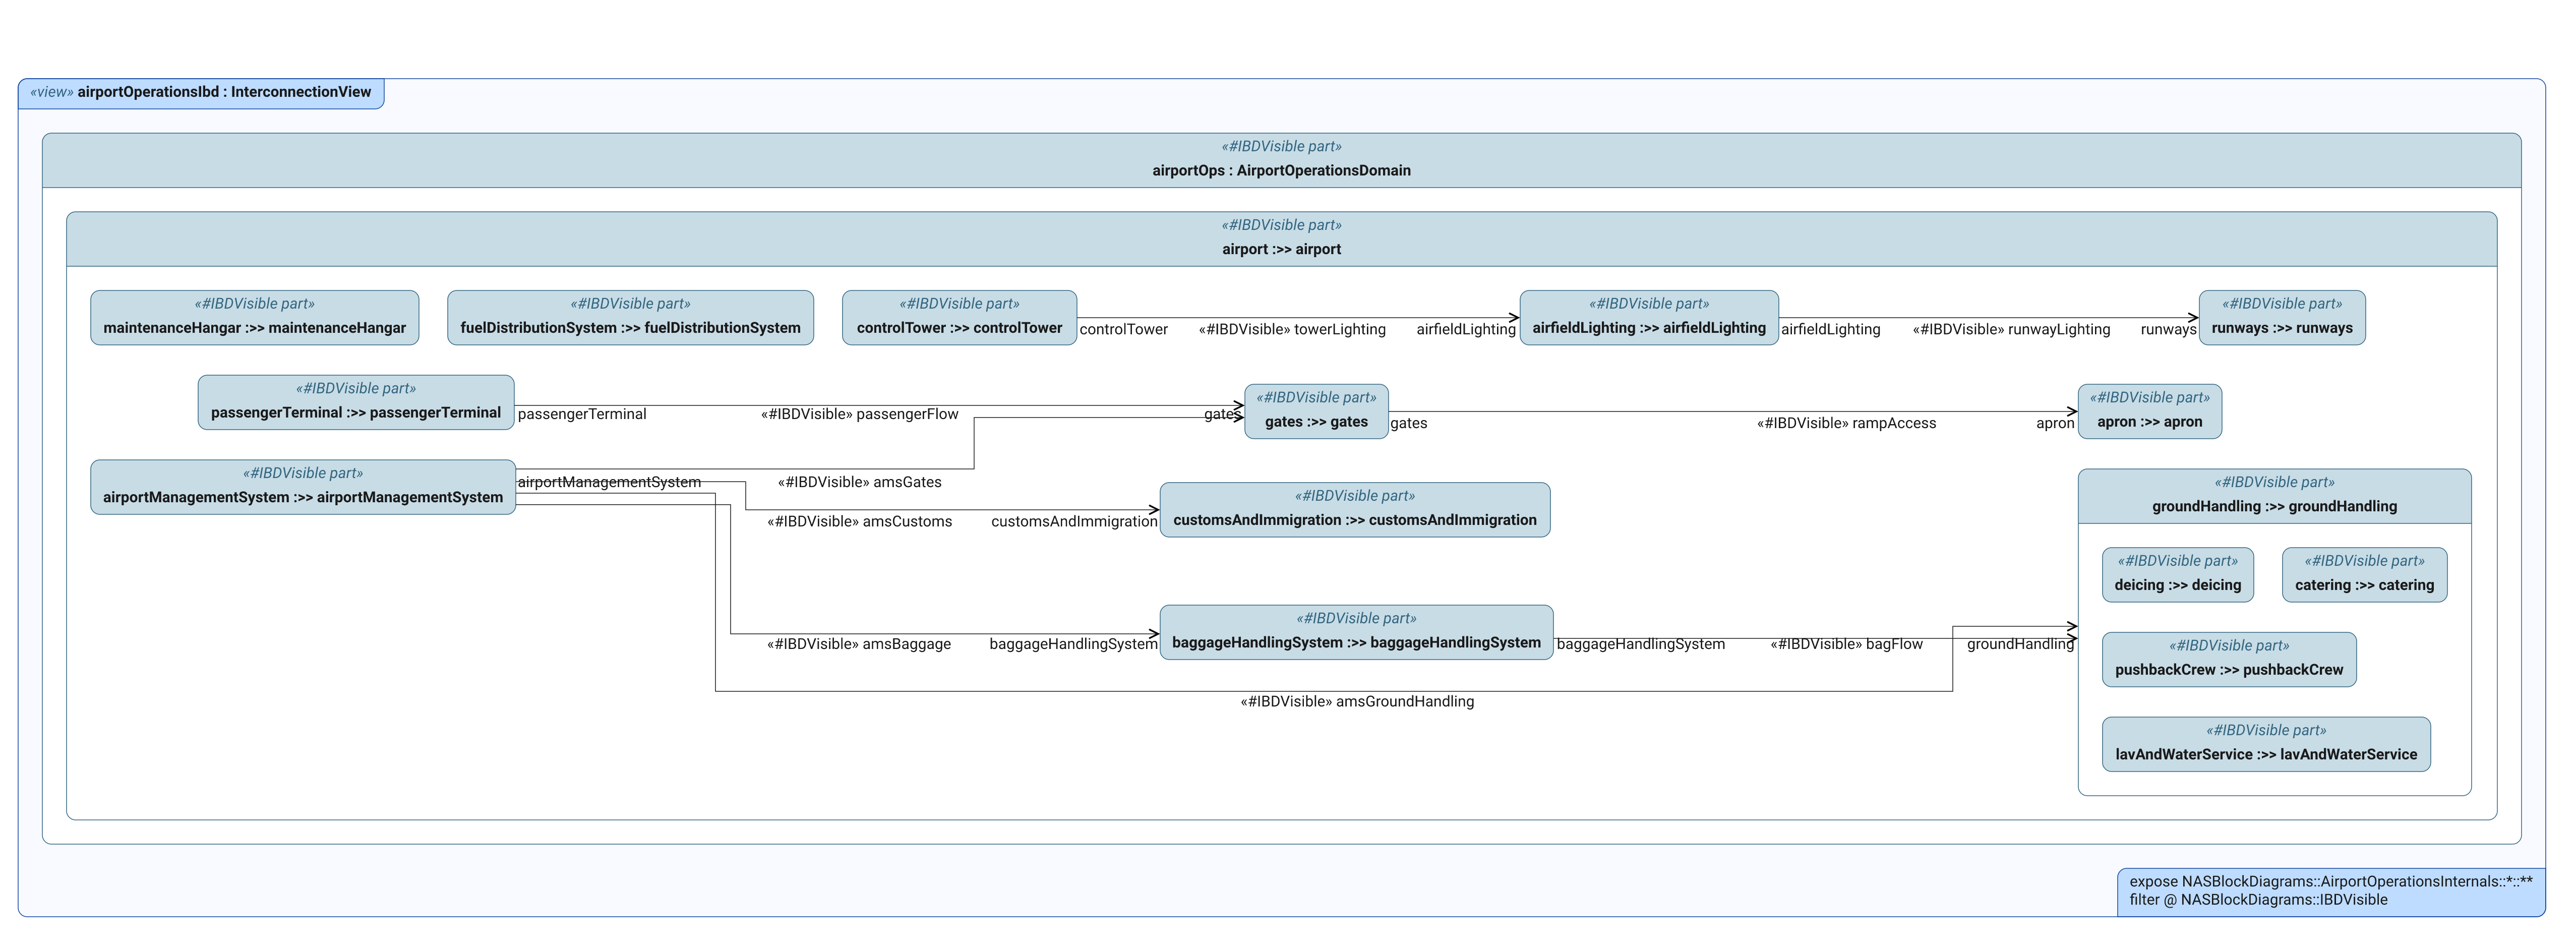
\includegraphics[width=\linewidth,height=0.8\textheight,keepaspectratio]{sysml/diagram-airportOperationsIbd}
\caption{Airport operations internal block diagram. View \texttt{airportOperationsIbd}; source \texttt{nas\_block\_diagrams.sysml}; rendered 2026-10-19.}
\label{fig:sysml-airportOperationsIbd}
\end{figure}
\end{landscape}

\begin{landscape}
\begin{figure}[!htbp]
\centering
\pdfimageresolution=300
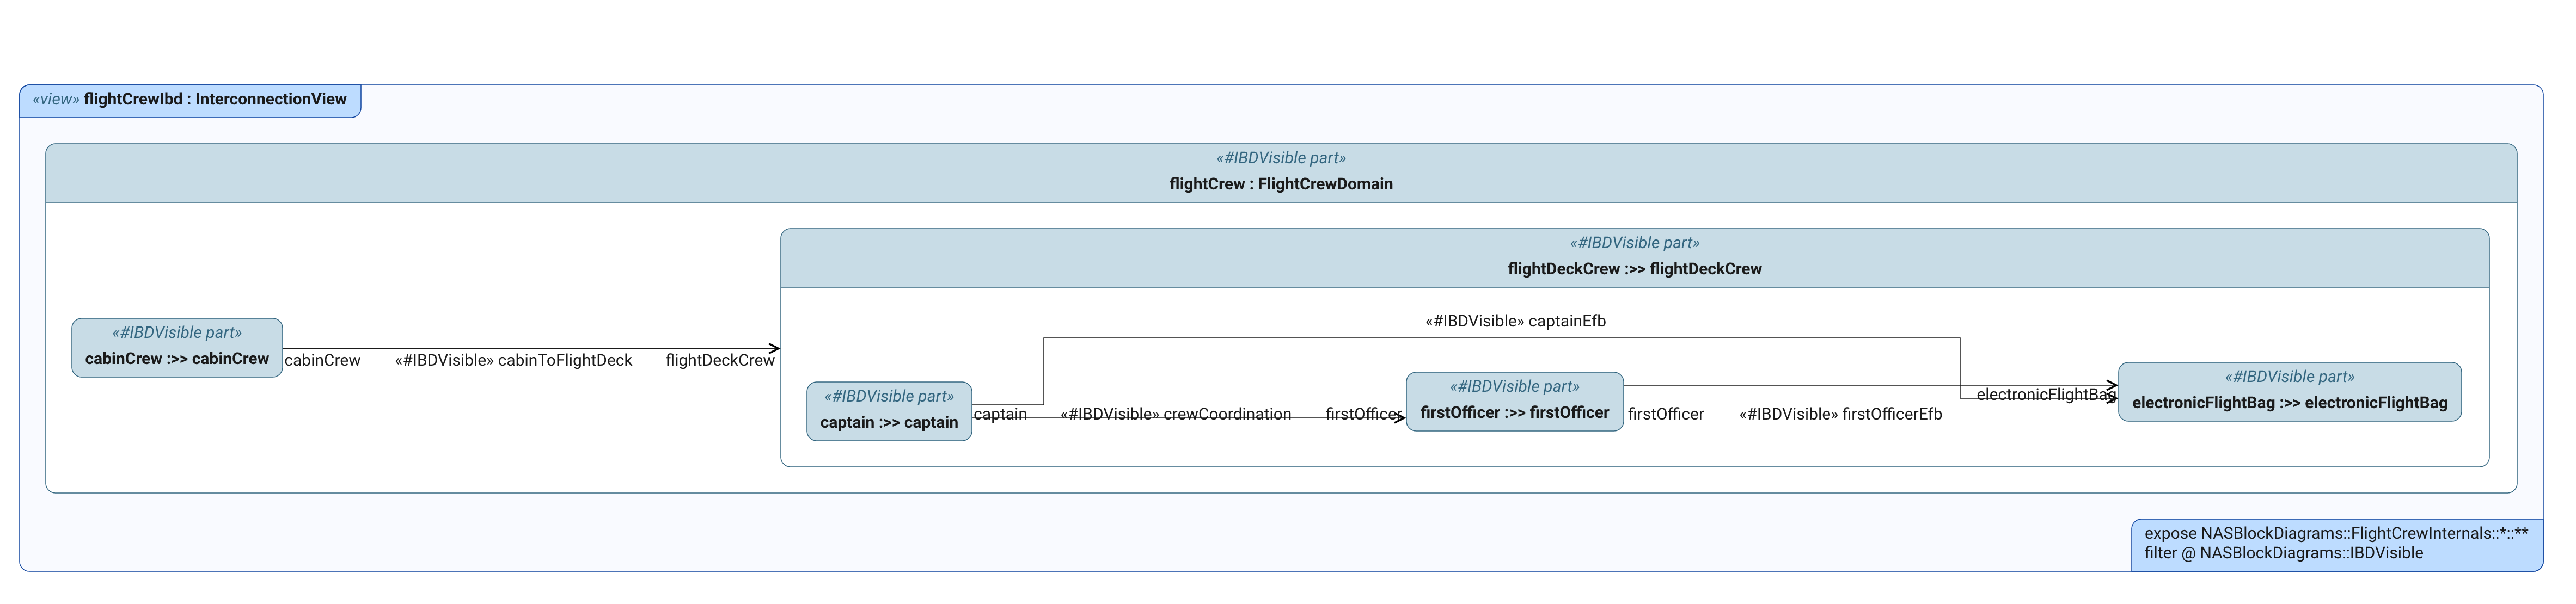
\includegraphics[width=\linewidth,height=0.8\textheight,keepaspectratio]{sysml/diagram-flightCrewIbd}
\caption{Flight crew internal block diagram. View \texttt{flightCrewIbd}; source \texttt{nas\_block\_diagrams.sysml}; rendered 2026-10-19.}
\label{fig:sysml-flightCrewIbd}
\end{figure}
\end{landscape}

\begin{landscape}
\begin{figure}[!htbp]
\centering
\pdfimageresolution=300
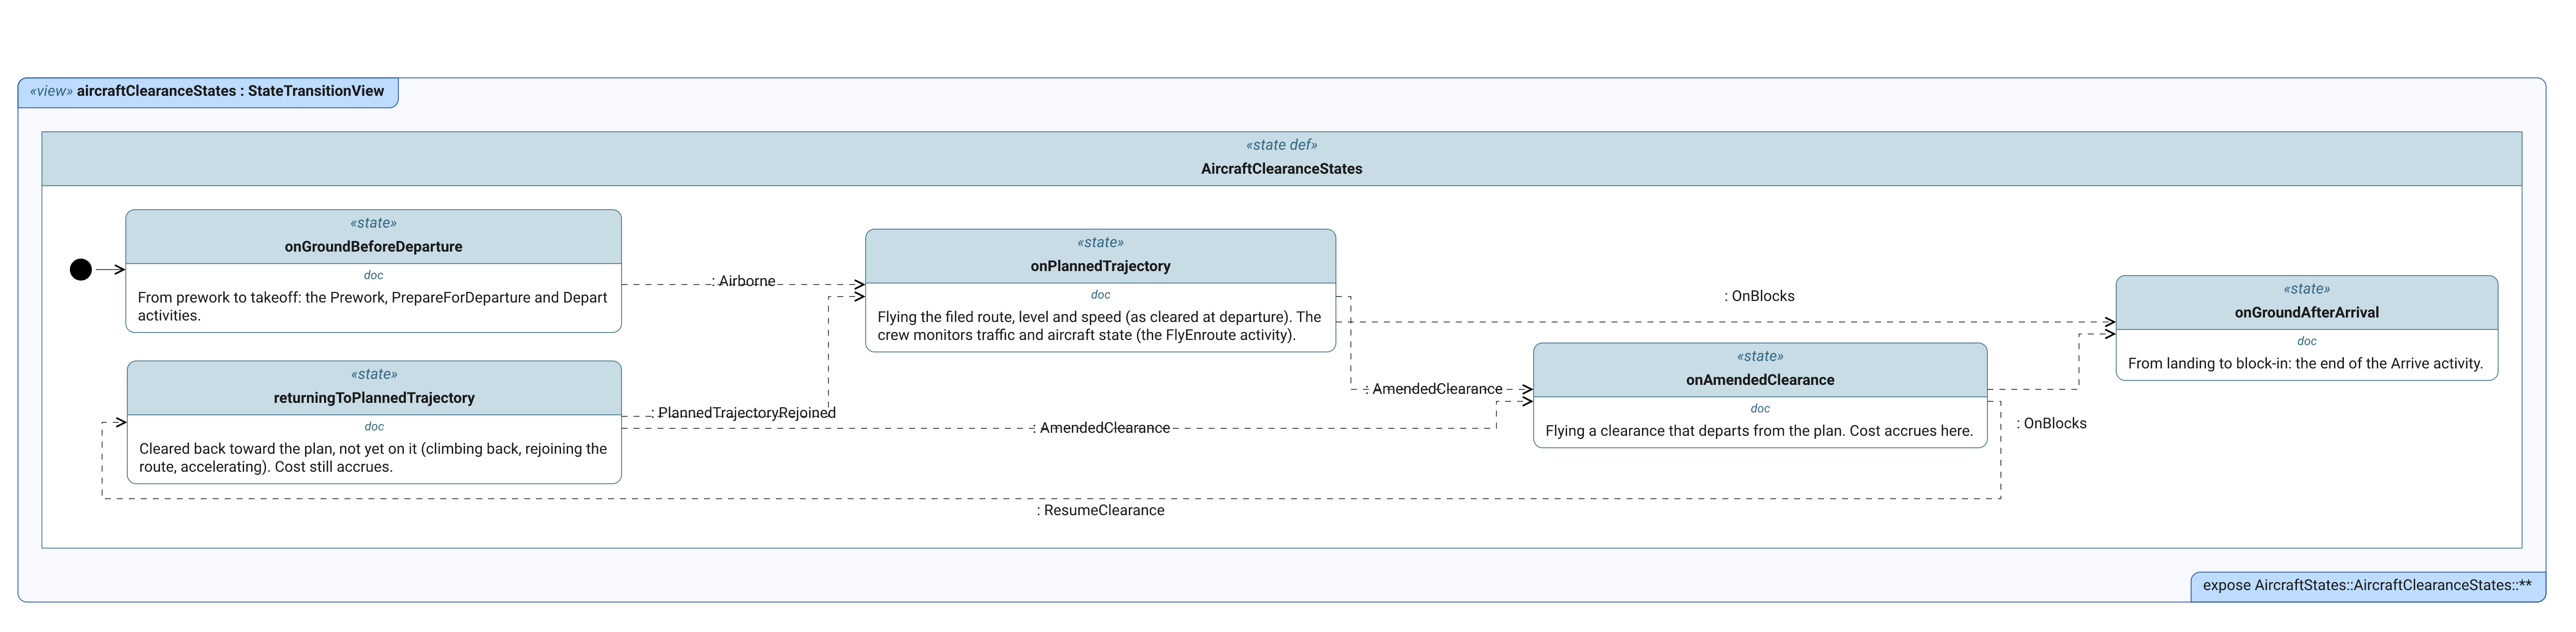
\includegraphics[width=\linewidth,height=0.8\textheight,keepaspectratio]{sysml/diagram-aircraftClearanceStates}
\caption{Aircraft state machine: the clearance the aircraft is flying, from the ground before departure to the ground after arrival. View \texttt{aircraftClearanceStates}; source \texttt{nas\_state\_aircraft.sysml}; rendered 2026-10-28.}
\label{fig:sysml-aircraftClearanceStates}
\end{figure}
\end{landscape}

\begin{landscape}
\begin{figure}[!htbp]
\centering
\pdfimageresolution=300
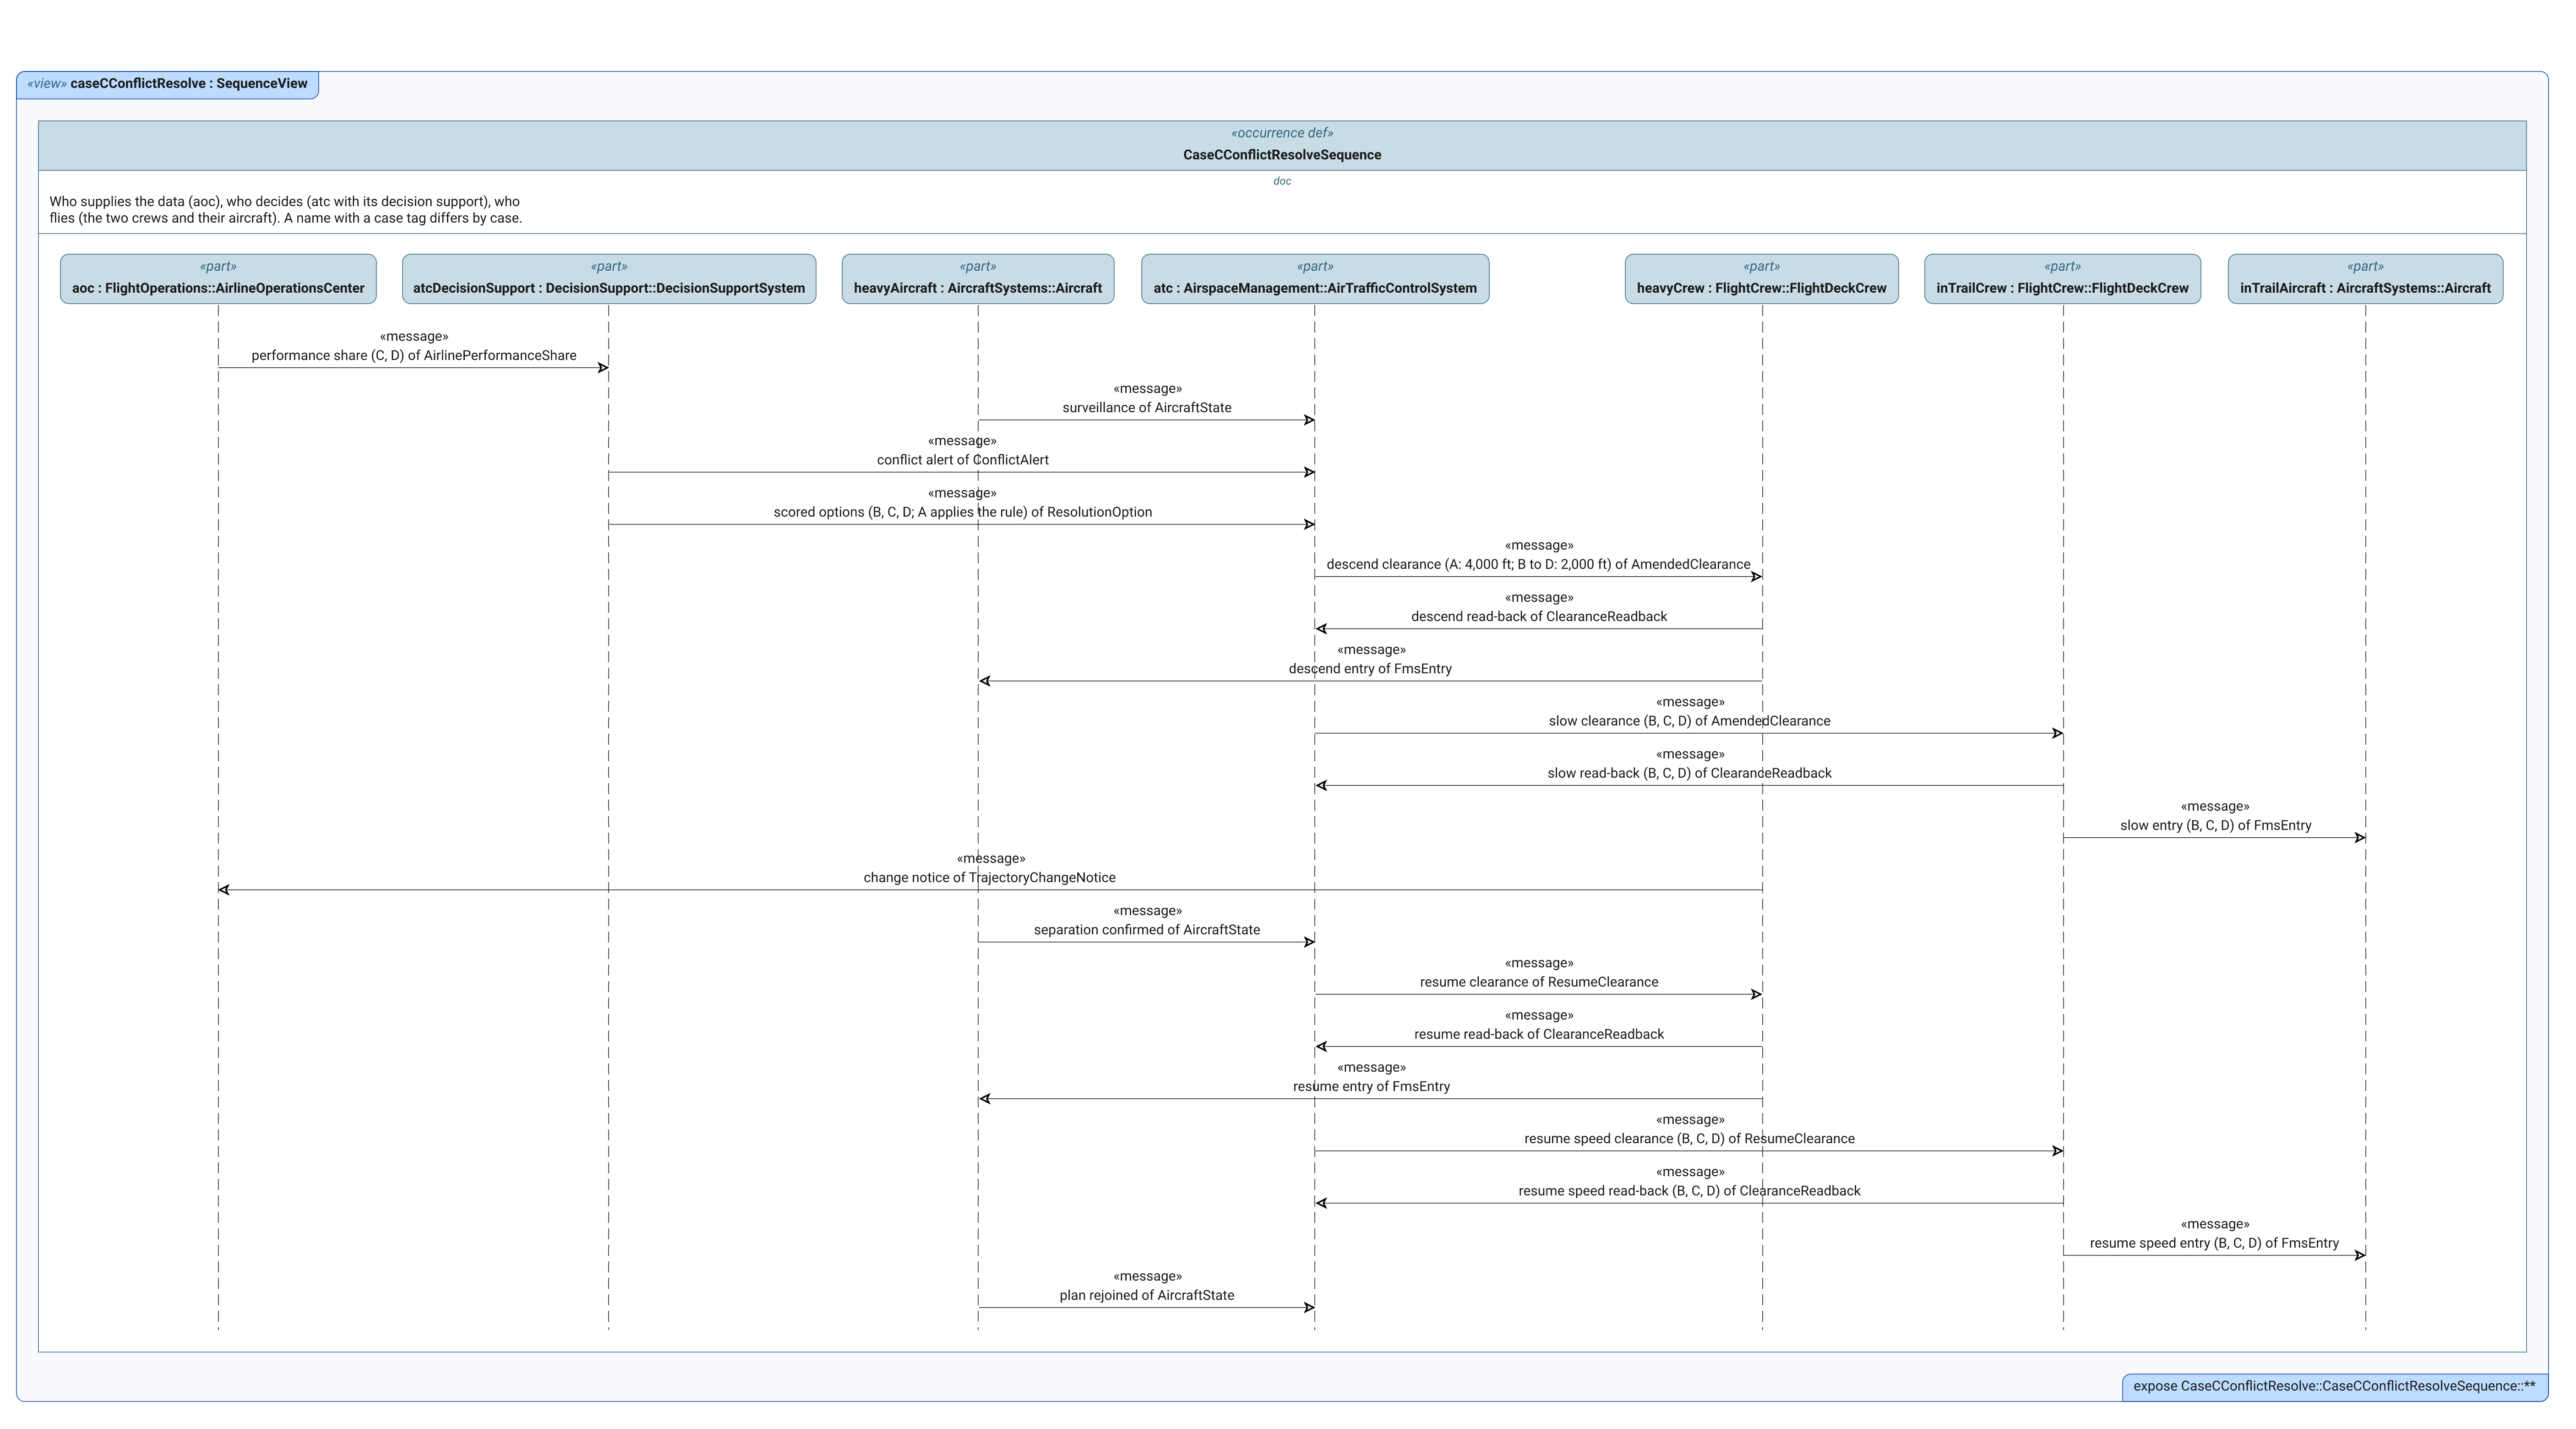
\includegraphics[width=\linewidth,height=0.8\textheight,keepaspectratio]{sysml/diagram-caseCConflictResolve}
\caption{Case C Conflict Resolve: the exchanges when ATC decision support scores the options with the airline's shared data. View \texttt{caseCConflictResolve}; source \texttt{nas\_sequence\_case\_c.sysml}; rendered 2026-10-28.}
\label{fig:sysml-caseCConflictResolve}
\end{figure}
\end{landscape}

\begin{landscape}
\begin{figure}[!htbp]
\centering
\pdfimageresolution=300
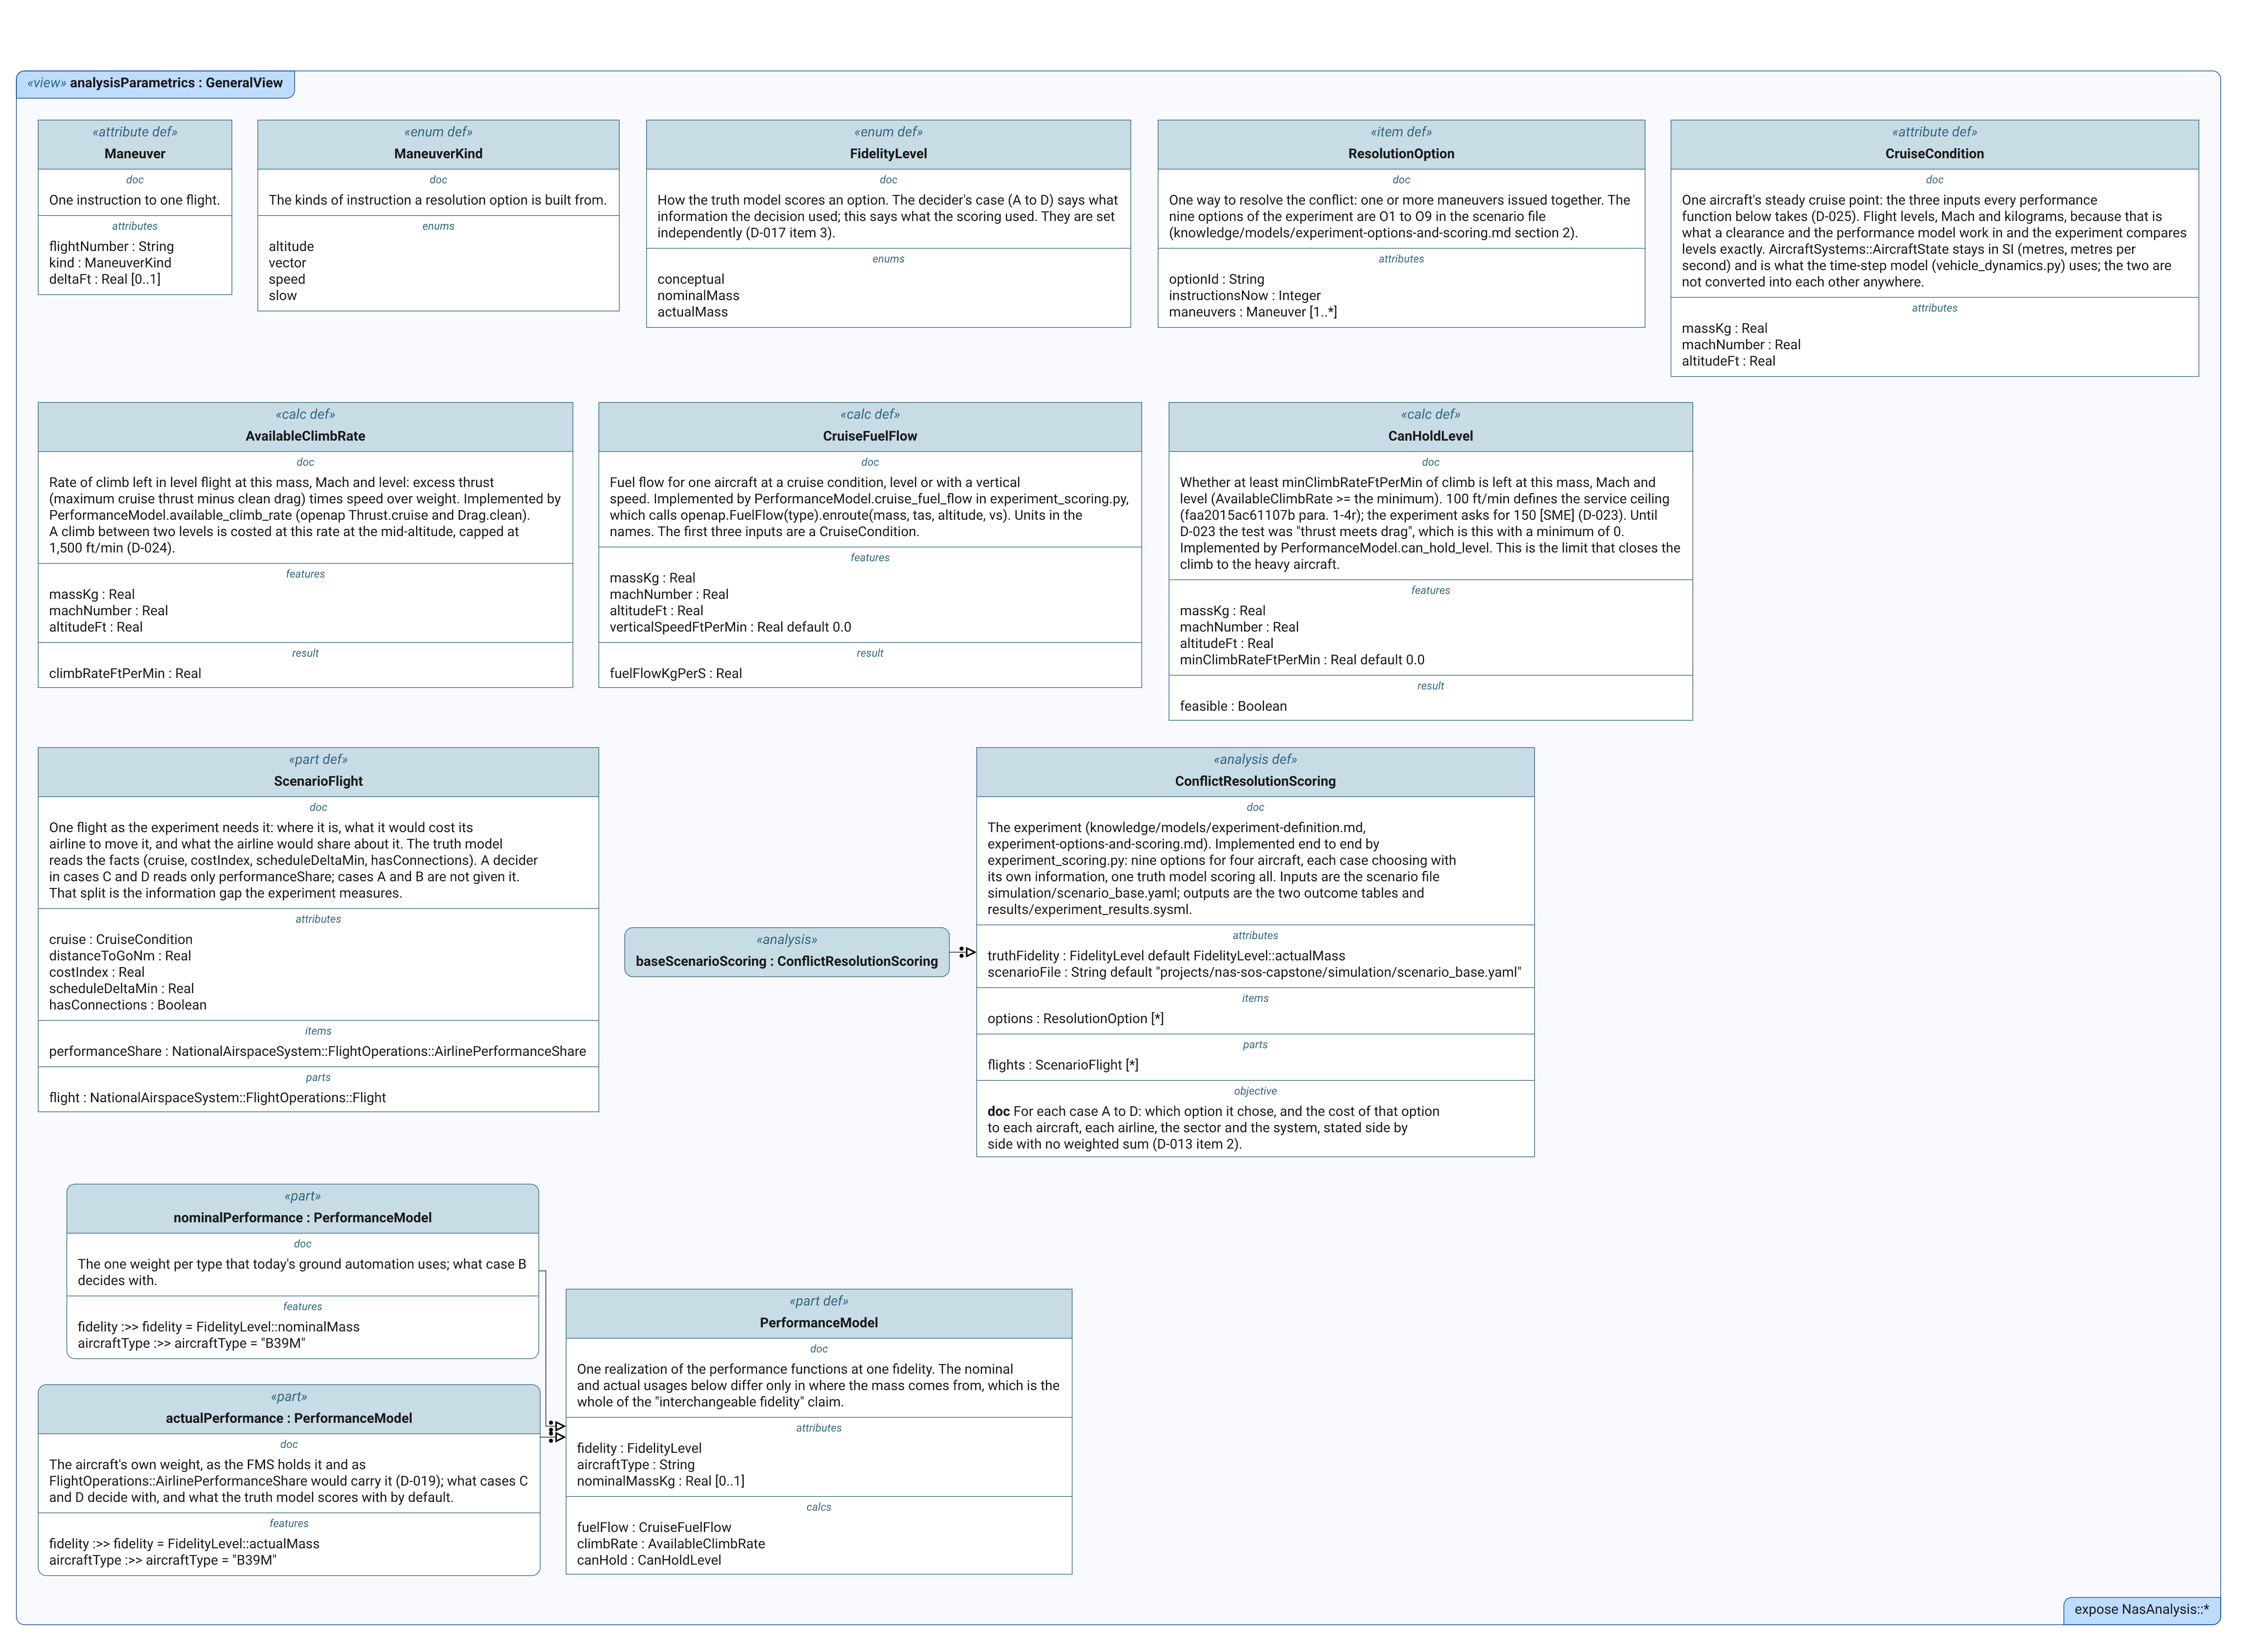
\includegraphics[width=\linewidth,height=0.8\textheight,keepaspectratio]{sysml/diagram-analysisParametrics}
\caption{Analysis definitions: the performance calculations, the two fidelity usages and the conflict-resolution scoring analysis. View \texttt{analysisParametrics}; source \texttt{nas\_analysis.sysml}; rendered 2026-10-28.}
\label{fig:sysml-analysisParametrics}
\end{figure}
\end{landscape}
